\begin{flushright} {\tiny {\color{gray} benchmark\_rtwave.tex}} \end{flushright}
%~~~~~~~~~~~~~~~~~~~~~~~~~~~~~~~~~~~~~~~~~~~~~~~~~~~~~~~~~~~~~~~~~~~~~~~~~~~~~~~

In Appendix D of \textcite{thie11} (2011) I wrote:
This benchmark is based on the analytical solution by \textcite{ramb68} (1968) 
and has been the subject of a numerical investigation by
\textcite{deka08} (2008). It consists of a two-layer system driven 
by gravity. No-slip boundary conditions are imposed on the
top and the bottom of the box, while free slip are imposed on
the sides. Fluid 1 ($\eta_1,\rho_1$) of thickness $h_1$ 
overlays fluid 2 ($\eta_2,\rho_2$) of thickness $h_2$ 
(with $h_1+h_2=L_y$).
An initial sinusoidal disturbance of the interface between these
layers is introduced and is characterised by an amplitude $\Delta$ and a
wavelength $\lambda = L_x/2$.

\begin{center}
\includegraphics[width=5cm]{images/rtwave/setup}
\end{center}

Under these conditions, the velocity of the diapiric growth $\upnu$ is
given by
\[
\frac{\upnu}{\Delta} = -K \frac{\rho_1-\rho_2}{2 \eta_2} h_2 g
\]
with $K$ being the dimensionless growth factor, function of
$\phi_1$, $\phi_2$, $\eta_1$ and $\eta_2$ 
with 
\[
K=\frac{-d_{12}}{c_{11}j_{22}-d_{12}i_{21}}
\]
and 
\begin{eqnarray}
c_{11} &=& \frac{\eta_1 2 \phi_1^2}{\eta_2(\cosh 2\phi_1 - 1 - 2\phi_1^2)} - \frac{2\phi_2^2}{\cosh 2\phi_2 - 1 - 2 \phi_2^2}\\
d_{12} &=& \frac{\eta_1(\sinh 2\phi_1 -2\phi_1)}{\eta_2(\cosh 2\phi_1 -1 -2\phi_1^2)} + \frac{\sinh 2\phi_2 - 2\phi_2}{\cosh 2\phi_2 -1 -2\phi_2^2} \\
i_{21} &=& \frac{\eta_1\phi_2 (\sinh 2 \phi_1 + 2 \phi_1)}{\eta_2(\cosh 2\phi_1 -1 -2\phi_1^2)} 
+ \frac{\phi_2 (\sinh 2\phi_2 + 2\phi_2)}{\cosh 2\phi_2 -1 -2\phi_2^2} \\
j_{22} &=& \frac{\eta_1 2 \phi_1^2 \phi_2}{\eta_2(\cosh 2\phi_1 -1-2\phi_1^2)} - \frac{2\phi_2^3}{ \cosh 2\phi_2 -1 -2\phi_2^2}\\
\phi_1&=&\frac{2\pi h_1}{\lambda}\\
\phi_2&=&\frac{2\pi h_2}{\lambda}
\end{eqnarray}
These equations are obtained from Section 20.2 of \textcite{gery19book}.

In \textcite{thie11} (2011) this benchmark is ran with 
$\rho_1=3300$, $\rho_2=3000$, $\eta_1=10^{21}$,
$\eta_2$ varied between $10^{19}$ and $10^{27}$
$L_x=500km$, $L_x$ varied between 500 and 1500km,
leading to $2\pi/3 \le \phi_1 \le 2\pi$.
A constant resolution of $75\times 75$ elements is chosen and each element contains
$5\times 5$ markers [particle in cell technique was used]. 
This set of measures is conducted for two values
of the perturbation amplitude:
$\Delta=h_y$ and $\Delta=h_y/3$.

\begin{center}
\includegraphics[width=6cm]{images/rtwave/thie11}\\
{\captionfont Taken from \textcite{thie11} (2011).}
\end{center}

This benchmark is carried out in \stone~40 with slightly 
different parameters, and also in \stone~120.


